\chapter{Spark RDD创建及转换}
\label{chap:rddcreate}
经过第\ref{scinitial}章SparkContext的初始化,Driver端会立即进行RDD的生成和转换。本章将按照WordCount实例对RDD生成和转换进行详解。
\section{Spark RDD综述}

RDD即为弹性数据集,它可以由存储在物理中的数据来生成,也可以通过其他RDD进行转换,RDD是Spark平台上的最基础的数据结构,分布式下可并行处理,并且对数据分区也可以根据业务不同进行改变,同时在系统内存资源足够的情况下,允许用户将计算中间结果缓存在内存中,后续的计算可以直接使用这个结果,这会极大的提高计算效能。

每个RDD内部,有下面5个主要的属性:

\begin{enumerate}[\bfseries 1]
	\item 数据分区列表
	
	为数据的基本组成单元,对于RDD来说,一个分区上将会对应一个计算任务,分区的个数会决定Job的并发度。在使用时可以由用户显示的指定分区数,没有指定的情况下,集群会采用默认的分区数,即集群工作节点上一个cpu core对应一个分区。分区的管理为BlockManager。
	\item 每个分区上的计算函数
	
	Spark中每个RDD都会实现一个computer函数,computer函数会对迭代器进行连接,但不会保存每次连接运算的中间结果。
	\item 对其他RDD的依赖列表
	
	RDD的每次转换都会生成一个新的RDD,新生成RDD(子RDD)会将旧RDD(父RDD)加入依赖,并将依赖加入列表中,这样就会形成一条线连接起各个RDD,这条线也称作生命线(lineage)。
	\item (可选)一个分区器
	
	针对key-value的RDD,分区器按照RDD的键值对进行处理,父RDD中的键值对在子RDD中分到哪个分区,分区器有两种,分变为HashPartitioner和RangePartitioner。分区器不但决定了RDD本身的分区数量,也决定了子RDD中输出的分区数量。
	\item (可选)计算每个分区优先位置列表
	
	对于数据源存储在HDFS中的,此列表存储的就是每个分区所在的块的位置。
\end{enumerate}
\section{Spark RDD创建}

创建RDD的方式有两种,第一种从存储在物理设备上的数据集创建,常见的有本地文件系统、HDFS和HBase,第二种通过已经存储在RDD进行转换。WordCount实例中数据存放在HDFS中,通过textFile读取HDFS文件内容并创建HadoopRDD。
\section{Spark RDD转换}

Spark RDD中的所有转换都是惰性的,在触发动作之前都只做单纯的连接。WordCount实例中,在RDD创建后通过flatmap生成一个新的数据集,并传入map生成新的数据集,接着传入reduceByKey,再接着传入filter生成新的数据集,最后返回给Driver的是saveAsText处理后的数据集,而不是整个数据集。
\section{DAG的生成}

Spark根据用户提交的计算逻辑中RDD的转换和动作来生成RDD之间的依赖关系,同时这个计算链条也就成了逻辑上的DAG。
\subsection{RDD中依赖}

RDD中每个Dependency子类内部都会存储一个RDD对象,对应一个父RDD,如果一次转换操作有多个父RDD,就会对应产生多个Dependency对象,使用List存储,所有的Dependency对象存储在子RDD内部,通过遍历RDD内部的Dependency对象,就能获取该RDD所有依赖的父RDD。RDD中主构造函数声明了Dependency的类型,如程序\ref{inputPrg:mainContruRDD}所示,可见RDD的deps为Seq类型,且其中的元素为Dependency。
\begin{codeInput}{Scala}{RDD主构造函数}{mainContruRDD}
abstract class RDD[T: ClassTag](
  @transient private var _sc: SparkContext,
  @transient private var deps: Seq[Dependency[_]]
  ) extends Serializable with Logging {
    ......
}
\end{codeInput}
子RDD和父RDD的依赖关系有两种,即宽依赖和窄依赖。两种依赖最简单的理解如图\ref{fig:deps}所示
\begin{enumerate}[\bfseries 1]
	\item 宽依赖是指子RDD中的一个分区依赖于父RDD的多个分区
	\item 窄依赖是指子RDD中的一个分区依赖于父RDD的一个分区
\end{enumerate}
\begin{figure}[H] 
	\centering
	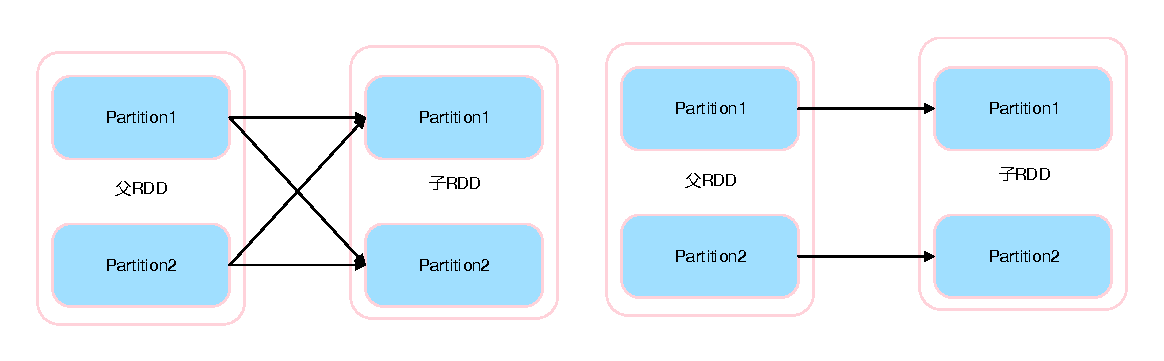
\includegraphics[width=\textwidth]{figures/wideandnarroewdeps.pdf}
	\caption{宽依赖(左)窄依赖(右)}
	\label{fig:deps}
\end{figure}

RDD不同的转换操作对应分区的映射规则不一样,但对于窄依赖而言计算任务作用于不同的数据分区,它们之间相互没有影响,所以这些计算任务也就可以并发的执行了。宽依赖中子RDD的单个分区要依赖父RDD的多个分区,因此这两个RDD不能通过一个计算任务来完成,这里需要进行shuffle。

RDD中依赖的层次图如图\ref{fig:depsclass}所示
\begin{figure}[H] 
	\centering
	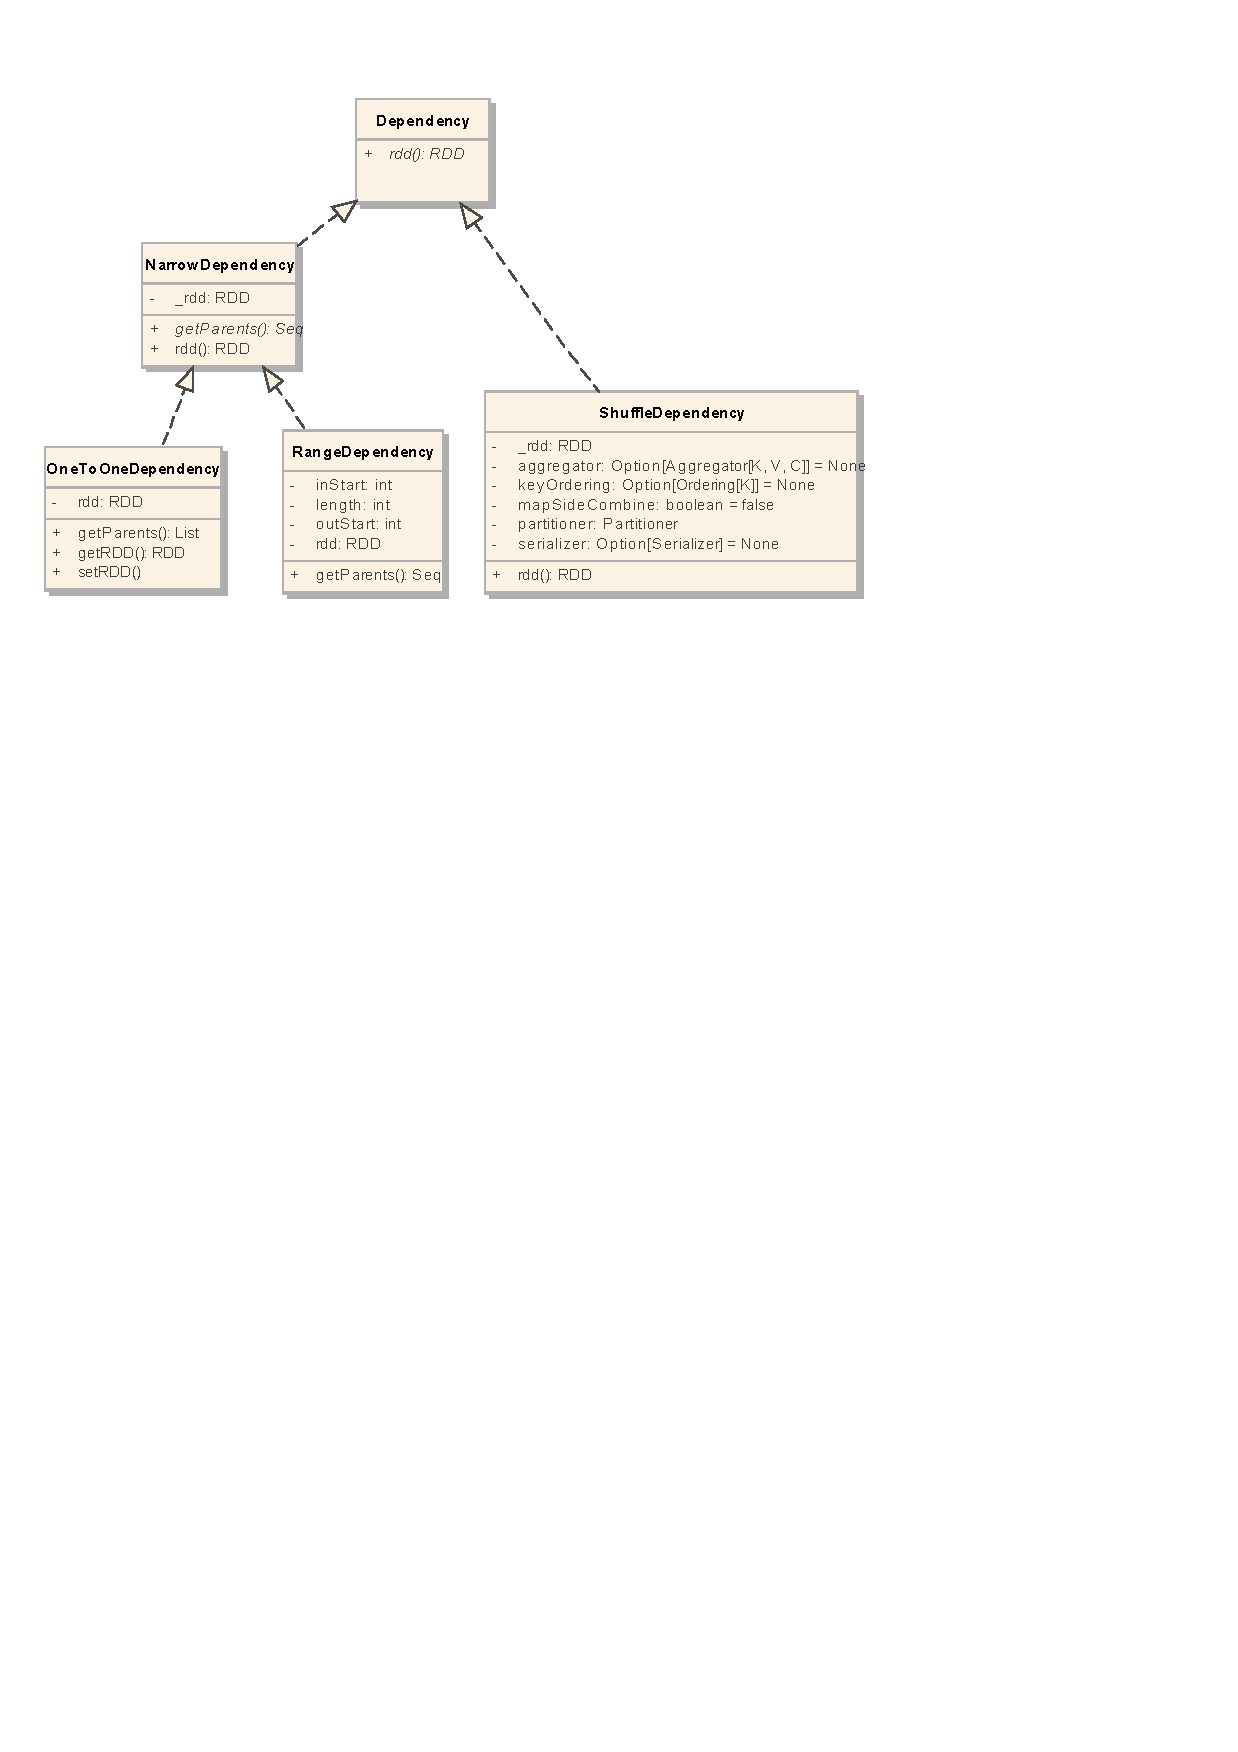
\includegraphics[width=\textwidth]{figures/dependencyclassl.pdf}
	\caption{Spark RDD依赖类层次图}
	\label{fig:depsclass}
\end{figure}
所有的依赖都要实现抽象类Dependency,其代码如程序\ref{inputPrg:abstractdeps}所示
\begin{codeInput}{Scala}{抽象类Dependency}{abstractdeps}
abstract class Dependency[T] extends Serializable {
  def rdd: RDD[T]
}
\end{codeInput}
这其中的rdd即为参数此RDD的父RDD,此为抽象方法,在子类中都必须有其实现。

窄依赖的实现如程序\ref{inputPrg:abstractnarrowdeps}所示
\begin{codeInput}{Scala}{NarrowDependency}{abstractnarrowdeps}
abstract class NarrowDependency[T](_rdd: RDD[T]) extends Dependency[T] {
  def getParents(partitionId: Int): Seq[Int]
  override def rdd: RDD[T] = _rdd
}
\end{codeInput}
这其中实现了对父RDD中rdd方法的实现,同时定义了一个抽象方法getParents,获取该依赖对应的父RDD的分区。

对于窄依赖的实现有两种,一种是OneToOneDependency,另一种是RangeDependency,这两种依赖都实现了getParents方法,只不过OneToOneDependency中父RDD和子RDD中的分区ID是相同的,RangeDependency仅仅被org.apache.spark.UnionRDD所使用,针对的是子RDD有多个父RDD的情形,但一对父子RDD中,分区任然是一对一,这种情形下依赖如图\ref{fig:rangedeps}所示
\begin{figure}[H] 
	\centering
	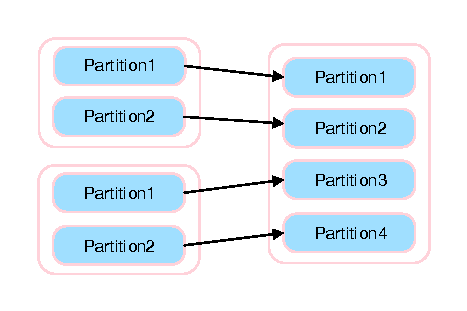
\includegraphics[scale=1.5]{figures/rangedeps.pdf}
	\caption{RangeDependency示例}
	\label{fig:rangedeps}
\end{figure}

宽依赖只有一种实现:ShuffleDependency,其代码如程序\ref{inputPrg:widedeps}所示
\begin{codeInput}{Scala}{ShuffleDependcy}{widedeps}
class ShuffleDependency[K: ClassTag, V: ClassTag, C: ClassTag](
  @transient private val _rdd: RDD[_ <: Product2[K, V]],
  val partitioner: Partitioner,
  val serializer: Option[Serializer] = None,
  val keyOrdering: Option[Ordering[K]] = None,
  val aggregator: Option[Aggregator[K, V, C]] = None,
  val mapSideCombine: Boolean = false)
    extends Dependency[Product2[K, V]] {	
      override def rdd: RDD[Product2[K, V]] = _rdd.asInstanceOf[RDD[Product2[K, V]]]
      private[spark] val keyClassName: String = reflect.classTag[K].runtimeClass.getName
      private[spark] val valueClassName: String = reflect.classTag[V].runtimeClass.getName
      private[spark] val combinerClassName: Option[String] =
      Option(reflect.classTag[C]).map(_.runtimeClass.getName)	
      val shuffleId: Int = _rdd.context.newShuffleId()
      val shuffleHandle: ShuffleHandle =
       _rdd.context.env.shuffleManager.registerShuffle(
        shuffleId,_rdd.partitions.size,this)
      _rdd.sparkContext.cleaner.foreach(
        _.registerShuffleForCleanup(this))
}
\end{codeInput}

这里处理了一些变量,为map端本地聚合做准备。shuffle的具体过程会在以后章节进行分析。
\subsection{DAG构建}

RDD通过一系列转换,会形成自己的依赖列表,列表中的每个依赖都会包含一个父RDD的对象,ShuffleRDD依赖中另外包含了分区器、序列化器、map端聚合等参数。这些信息提供了子RDD由那些父RDD转换而来以及它所依赖的父RDD的分区信息。逻辑上,各RDD通过一条线连接,且由子RDD指向父RDD,这样就形成了一条Lineage,也可看做这些RDD形成了DAG。

Spark根据由DAG来划分Stage,进而生成计算任务。在同一个分区上进行计算的任务可以放在一个线程中计算,而宽依赖中子RDD要从父RDD的各个分区中拉取数据,并且放到不同的分区中进行计算,所以得新开一个线程进行。由此可得出划分Stage的依据就是ShuffleDependency。划分阶段在RDD触发Action之后,具体分析会在调度章节进行说明。

\subsection{WordCount的RDD转换和DAG生成}

本实例中WordCount运行在三台主机构成的集群中,两台为NodeManager ,一台作为ResourceManager,输入数据保存在HDFS上,且存在DataNode中的某一台上,RDD转换的细节如图\ref{fig:SparkCountDetails}所示
\begin{figure}[H] 
	\centering
	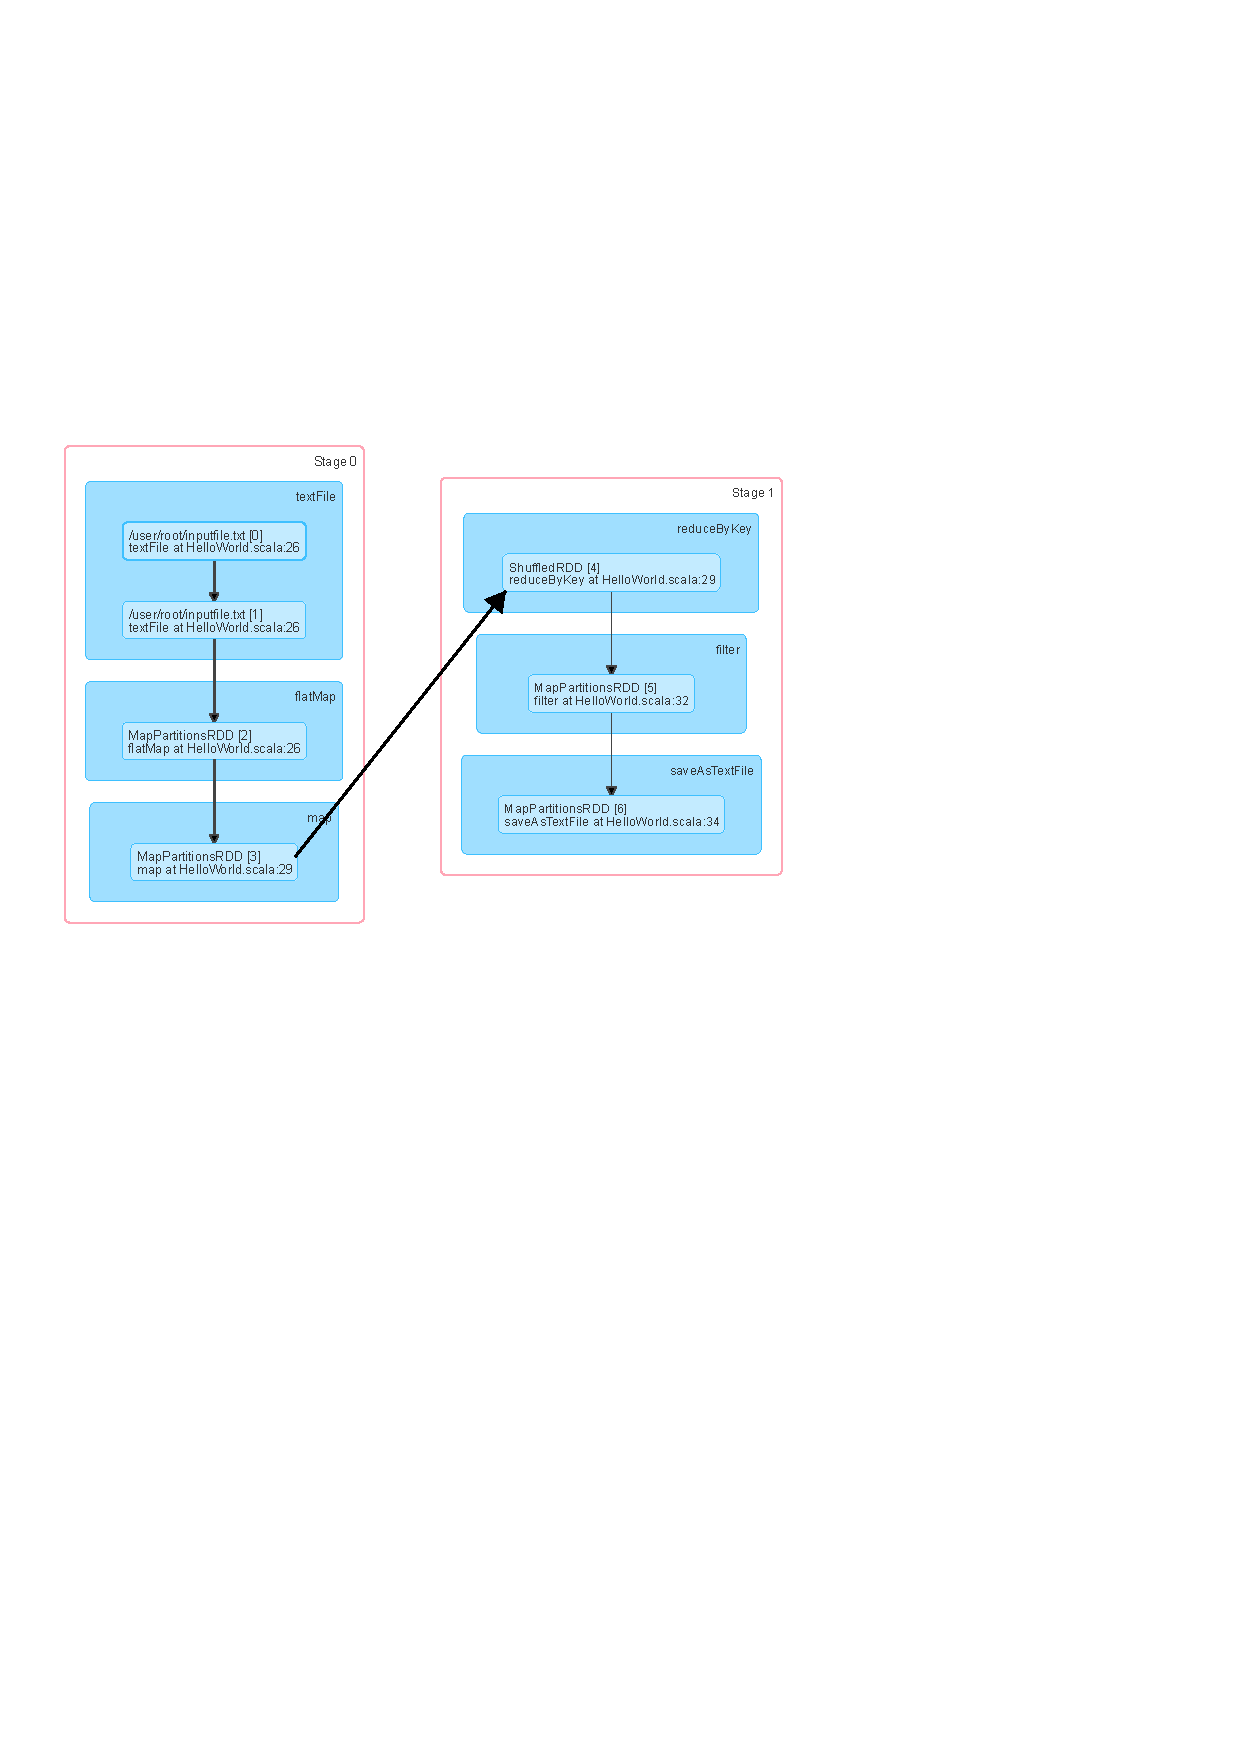
\includegraphics[width=\textwidth]{figures/SparkCountDetails.pdf}
	\caption{WordCount的RDD转换}
	\label{fig:SparkCountDetails}
\end{figure}

通过图\ref{fig:SparkCountDetails},可以清晰的看到数据被分成了两个分区,程序使用的默认分区数,即一个cpu core对应一个分区。用户对应的每一个操作会对应生成一个RDD,但对应shuffle操作如图中的reduceByKey会隐式的读在map端和reduce端分别产生一个MapPartitionRDD,中间生成一个shuffldedRDD,不过这些都是Spark内部进行的,用户不用关心。

为了加深对图\ref{fig:SparkCountDetails}中RDD的转换关系的理解,图\ref{fig:wordcountdatastream}描述了在本WordCount实例中真实数据下的转换和计算过程。
\begin{figure}[H] 
	\centering
	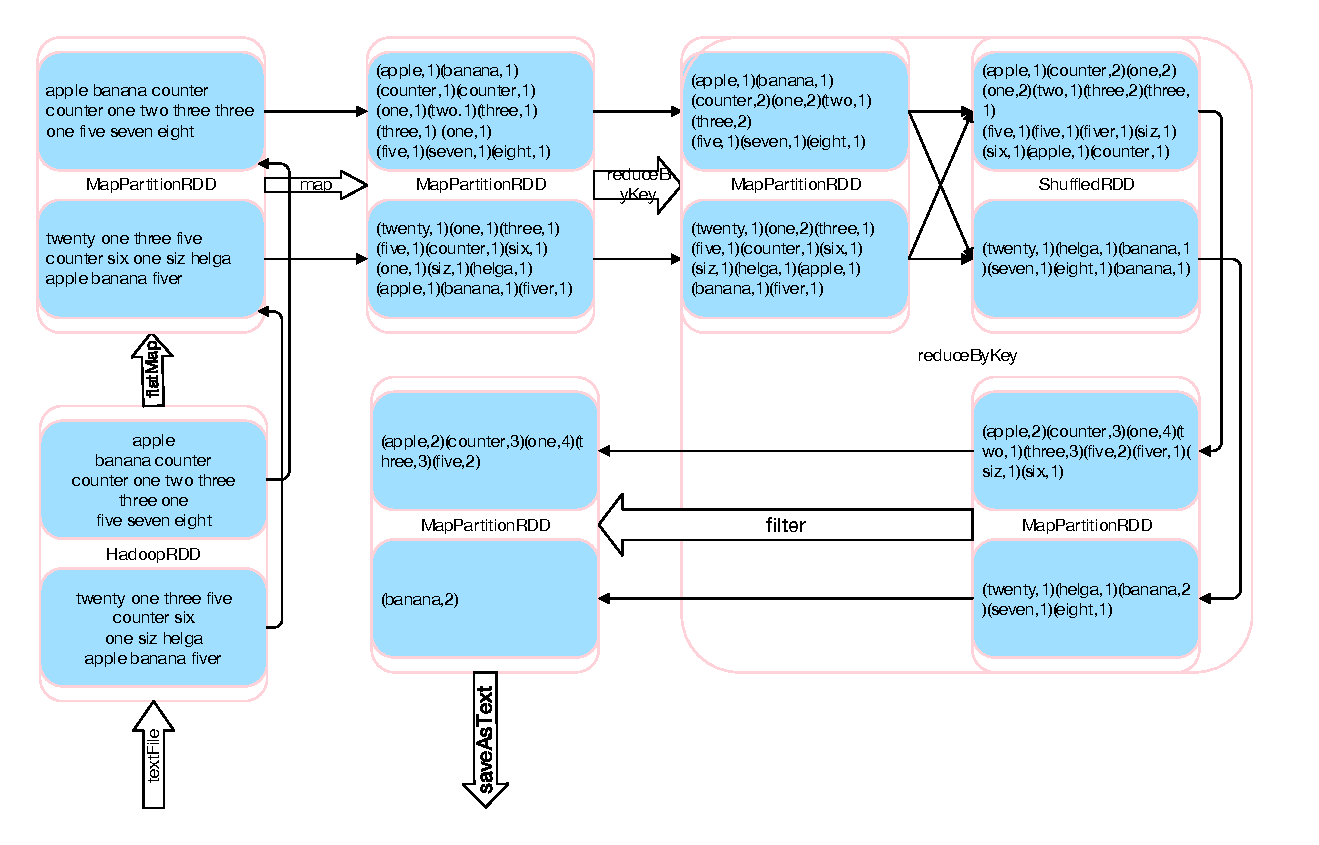
\includegraphics[width=\textwidth]{figures/wordcountdatastream.pdf}
	\caption{WordCount的数据逻辑图}
	\label{fig:wordcountdatastream}
\end{figure}

源数据存放在HDFS中,通过texFile读取后形成两个分区的HadoopRDD,这里是因为测试集群中总共两个cpu core,分区数设置为默认分区。这里也应该注意到在reduceByKey操作中,Spark产生了三个RDD,第一个为本地聚合后形成的MapPartitionRDD,第二个为通过网络操作按照分区器所设置的记录和子RDD中分区对应关系,将父RDD中相关记录拉取到子RDD中,此部分需要网络,也需要跨分区,这部分为性能调优的重点。最后一个RDD为reduce端聚合。